%
% \documentclass[fullscreen=true, bookmarks=false]{beamer}
% \usepackage[cp1251]{inputenc}
%\usepackage[english,russian]{babel}
%\usepackage{xcolor}
% \usepackage{wrapfig}
%\usetheme{Goettingen}
% \usetheme{Warsaw}
%\usecolortheme{beetle}
%\setbeamercovered{transparent}
%\setbeamertemplate{blocks}[rounded]% [shadow=false]
%\setbeamertemplate{frames}[shadow=false]

%\usebackgroundtemplate{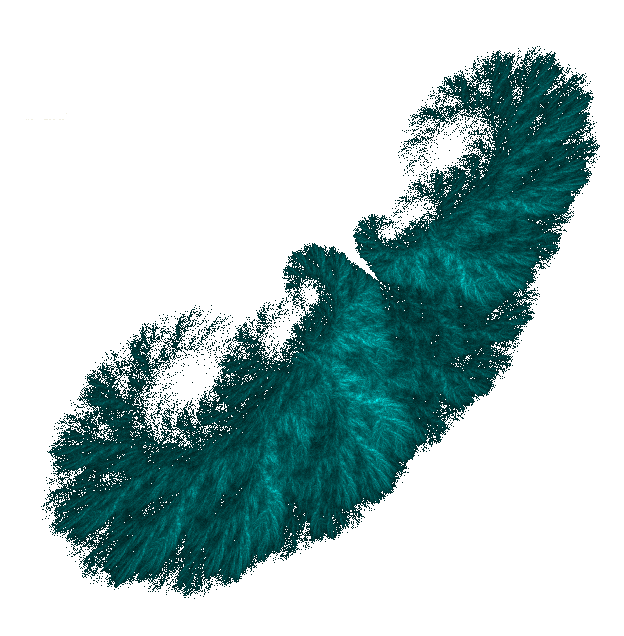
\includegraphics[width=\paperwidth,height=\paperheight,  keepaspectratio]{beamer1_biw.PNG}}
%
% \usebackgroundtemplate{\centering
%         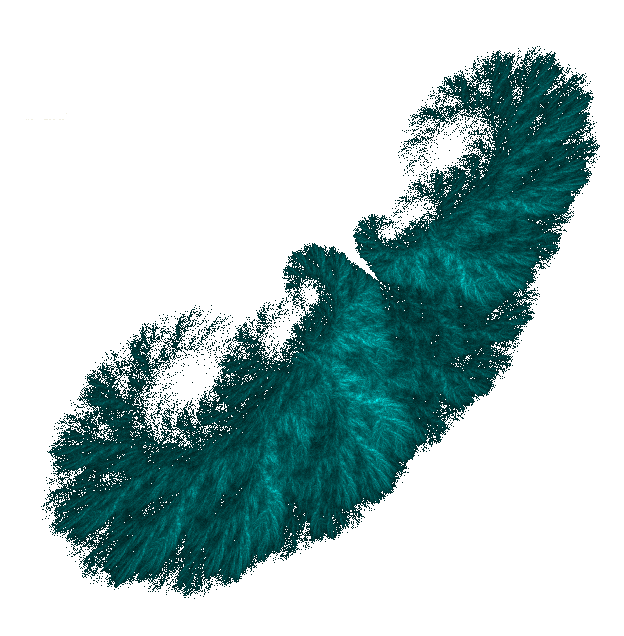
\includegraphics[height=7cm, keepaspectratio]{beamer1_biw.PNG}}

%\addtobeamertemplate{frame begin}{\pgfsetfillopacity{0.7}}{\pgfsetfillopacity{1}}
%\addtobeamertemplate{block begin}{\pgfsetfillopacity{0.7}}{\pgfsetfillopacity{1}}
% \title{Introduction to N-adic numbers}
% \subtitle{Practical Applications}
% \author{Denis Morozov}
% \institute{Samsung R\&D}
% \date{\today}

% %\setbeamercolor{color1}{fg = white}
% %\setbeamercolor{block title}{bg=red!30,fg=black}
% %\setbeamercolor{block body}{bg=red!30,fg=blue}

% \begin{document}

% \begin{frame}
% \titlepage
% \end{frame}

% \begin{frame}
% \begin{figure}[h]
% \center{\includegraphics[width=10em]{fomenko_solenoid.jpg}}
% \caption{A.Fomenko, 2-adic solenoid}
% \label{ris:image}
% \end{figure}
% %\centering \hspace{4em}\includegraphics[width=10em, keepaspectratio]{fomenko_solenoid.jpg}
% \end{frame}
% \begin{frame}
% \begin{block}{Introduction}

% \end{block}
% \end{frame}

% \end{document}
% $Header: /Users/joseph/Library/texmf/tex/latex/beamer/solutions/conference-talks/conference-ornate-20min.en.tex,v 90e850259b8b 2007/01/28 20:48:30 tantau $

\documentclass{beamer}

% This file is a solution template for:

% - Talk at a conference/colloquium.
% - Talk length is about 20min.
% - Style is ornate.



% Copyright 2004 by Till Tantau <tantau@users.sourceforge.net>.
%
% In principle, this file can be redistributed and/or modified under
% the terms of the GNU Public License, version 2.
%
% However, this file is supposed to be a template to be modified
% for your own needs. For this reason, if you use this file as a
% template and not specifically distribute it as part of a another
% package/program, I grant the extra permission to freely copy and
% modify this file as you see fit and even to delete this copyright
% notice. 


\mode<presentation>
{
  %\usetheme{CambridgeUS}
%\usetheme{Bergen}
%\usetheme{PaloAlto}
\usetheme{Warsaw}
  % or ...

  \setbeamercovered{transparent}
  % or whatever (possibly just delete it)
}


\usepackage[english]{babel}
% or whatever



\usepackage{times}
\usepackage[T1]{fontenc}
% Or whatever. Note that the encoding and the font should match. If T1
% does not look nice, try deleting the line with the fontenc.
%\usepackage{geometry} % to change the page dimensions
\usepackage{graphicx} % support the \includegraphics command and options
%\usepackage{pst-plot,pstricks-add}
%\usepackage[latin1]{inputenc}
\usepackage{tikz}

\usepackage{verbatim}
\usetikzlibrary{arrows,shapes}


\title[Introduction to N-adic numbers] % (optional, use only with long paper titles)
{Introduction to N-adic numbers}

\subtitle
{Practical Applications}


\author[Denis Morozov, PhD \ Samsung R\&D] % (optional, use only with lots of authors)
{Denis~ Morozov, PhD  \\  \texttt{morozov.den@samsung.com}}
% - Give the names in the same order as the appear in the paper.
% - Use the \inst{?} command only if the authors have different
%   affiliation.
\institute[Samsung R\&D] % (optional, but mostly needed)
{
  \inst{1}%
  Samsung R\&D
  \and
  \inst{2}%
  Department of Computer Science, doctoral studies\\
  University of "Kiev-Mogyla Academy"}
%  \and
% \vspace{.5cm}
 % \inst{3}%
  % \texttt{ formulation of the problem}

  %  \texttt{Valentin Vovk},  \texttt{ Mobile Lab 2}}
% - Use the \inst command only if there are several affiliations.
% - Keep it simple, no one is interested in your street address.

\date[February, 2013] % (optional, should be abbreviation of conference name)
{Presentation , 2013}
% - Either use conference name or its abbreviation.
% - Not really informative to the audience, more for people (including
%   yourself) who are reading the slides online

\subject{N-adic numbers course}
% This is only inserted into the PDF information catalog. Can be left
% out. 

\AtBeginSubsection[]
{
  \begin{frame}<beamer>{Outline}
    \tableofcontents[currentsection,currentsubsection]
  \end{frame}
}


% If you wish to uncover everything in a step-wise fashion, uncomment
% the following command: 

%\beamerdefaultoverlayspecification{<+->}


\begin{document}

\begin{frame}
  \titlepage
\end{frame}

\begin{frame}{Outline}
  \tableofcontents
  % You might wish to add the option [pausesections]
\end{frame}


% Structuring a talk is a difficult task and the following structure
% may not be suitable. Here are some rules that apply for this
% solution: 

% - Exactly two or three sections (other than the summary).
% - At *most* three subsections per section.
% - Talk about 30s to 2min per frame. So there should be between about
%   15 and 30 frames, all told.

% - A conference audience is likely to know very little of what you
%   are going to talk about. So *simplify*!
% - In a 20min talk, getting the main ideas across is hard
%   enough. Leave out details, even if it means being less precise than
%   you think necessary.
% - If you omit details that are vital to the proof/implementation,
%   just say so once. Everybody will be happy with that.

\section{Motivation}

\subsection{Objective}

\subsection{Basic Properties}

\begin{frame}{Sufficiency}
  % - A title should summarize the slide in an understandable fashion
  %   for anyone how does not follow everything on the slide itself.
 Consideration for the following reasons ultrametrics (non-Archimedean metric spaces) is natural:
  \begin{itemize}
  \pause
  \item
in the context of a real analysis of the computer is a discrete system, but in terms of a 2-adic - continuous
     
  \pause
  \item
the modern computer is essentially an analog in terms of non Archimedean analysis
    
  \end{itemize}


\end{frame}

\begin{frame}{Quick calculations}
  % - A title should summarize the slide in an understandable fashion
  %   for anyone how does not follow everything on the slide itself.

 2-adic continuity of the basic operations of the processor allows the creation of models that use floating point numbers, and all calculations are made   in the set of integers.

 \begin{itemize}
 \pause
  \item

 32 bit integer algorithms have good specifications for optimizing on existing processors
 \item
 \pause
 number-theoretical Fourier transform works well for convolutions with large kernels
  \end{itemize}

\end{frame}

% \begin{frame}{}

%   You can create overlays\dots
 %   \begin{itemize}
%   \item using the \texttt{pause} command:
%     \begin{itemize}
%     \item
%       First item.
%       \pause
%     \item    
%       Second item.
%     \end{itemize}
%   \item
%     using overlay specifications:
%     \begin{itemize}
%     \item<3->
%       First item.
%     \item<4->
%       Second item.
%     \end{itemize}
%   \item
%     using the general \texttt{uncover} command:
%     \begin{itemize}
%       \uncover<5->{\item
%         First item.}
%       \uncover<6->{\item
%         Second item.}
%     \end{itemize}
%   \end{itemize}
% \end{frame}


% \subsection{Previous Work}

% \begin{frame}{The Required Basic Information}{Power of Algebra and Number Theory}
% We were studied classical works using algebraic methods for calculating the convolution.
%  Different techniques, including the arithmetic of finite fields, linear algebra and group theory have been used.
% \pause


%  They were adapting to the implementation of algorithms for discrete convolution in C++ language
%  based processor architecture.
% \end{frame}





\section{Results}

\subsection{Main Results}

\begin{frame}{Main Result}{  \texttt{ formulation of the problem Valentin Vovk},  \texttt{ Mobile Lab 2}}
Implemented a two-dimensional convolution with algebraic methods for the size of $2^n\times 2^m$

\pause
 \begin{itemize}
 \item 
 $0 \leqslant m,n  \leqslant 10 $.
 \end{itemize}

\end{frame}



\begin{frame}{Plot Test Results}{   \texttt{tests conducted by Andrei Zavorotny},  \texttt{ Mobile Lab 2}}
%seen as a convolution made by algebraic methods give better results on large sizes
As we see algebraic methods for convolution yield the best results on large sizes
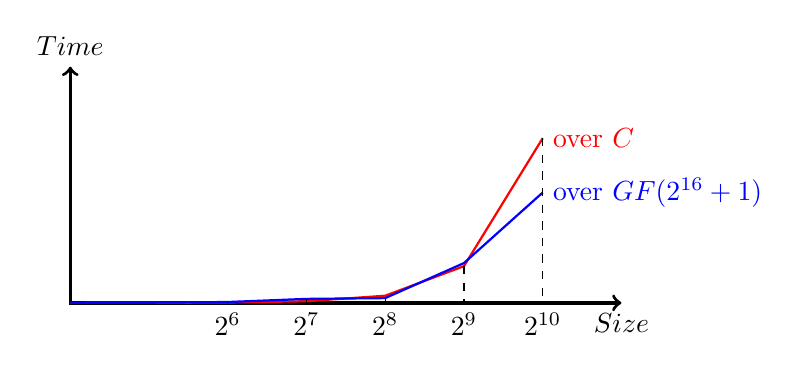
\begin{tikzpicture}
\draw[very  thick,  <->]  (7,0)  node[below]  {$Size$}
-|  (0,3)  node[above]  {$Time$};
\draw[red,  thick]  (0,0.0005) -- (1,0.00142) -- (2,0.00513) -- (3,0.02117) -- (4,0.09127) -- (5,0.467)-- (6,2.092)
node[right]  { over $\mathbb{C}$};
\draw[blue,  thick]  (0,0.0011) -- (1,0.00261) -- (2,0.01141) -- (3,0.05105) -- (4,0.06112) -- (5,0.506)-- (6,1.402)
node[right]  { over $GF(2^{16}+1)$};
% \draw[blue,  thick]  (1.5,4.5)  parabola[bend  at  end]
% (4.5,1.5)  node[right]  {$D $};
\draw[dashed]    (6,2.092)  node[left]  {}  -- (6,0)  node[below]  {$2^{10}$}

(5,0.467)  node[left]  {}  -- (5,0)  node[below]  {$2^{9}$}
(4,0.06112)  node[left]  {}  -- (4,0)  node[below]  {$2^{8}$}
(3,0.05105)  node[left]  {}  -- (3,0)  node[below]  {$2^{7}$}
(2,0.01141)  node[left]  {}  -- (2,0)  node[below]  {$2^{6}$}
;
% \draw[dashed]    (0,2.2)  node[left]  {$P_2$}  --
% (3.1,2.2)  (3.1,2.2)  --  (3.1,0)  node[below]  {$Q_2$};
\end{tikzpicture}
\end{frame}

\begin{frame}{Test Results}
  \begin{itemize}
 \item  
 Test results for large sizes
 \end{itemize}
\pause
  \hspace*{70pt}
\begin{tabular}{|c|c|c|c|}
\hline
 Size  & 1024 & 512 & 256  \\
\hline
\hline
 Furie  & 2092 & 467 & 91.27 \\
\hline
 Ferma  & 1402 & 506 & 61.12 \\

\hline
\end{tabular}

\end{frame}

\subsection{Basic Ideas for Implementation}

\begin{frame}{Base  Technical Points}

 During construction of the algorithm we are
  \begin{itemize}

\item
 reducing the number of using  modulo field's size

\pause
\item
 using the FFT algoritm of length 32 based on symmetry of transform matrix
\pause
\item
transition from 64-bit to 32-bit arithmetic

  \end{itemize}

\end{frame}


\begin{frame}
\frametitle{Cooley-Tukey scheme for for FFT}


\tikzstyle{format} = [regular polygon,regular polygon sides=9, draw, thin, fill=blue!20]
%\tikzstyle{format} = [diamond, draw, thin, fill=blue!20]
\tikzstyle{formatRed} = [ draw, thin, fill=red!20]
\tikzstyle{mediumGreen} = [ellipse, draw, thin, fill=green!20, minimum height=2.5em]
\tikzstyle{mediumRed} = [ellipse, draw, thin, fill=red!20, minimum height=2.5em]
\tikzstyle{mediumOrange} = [ellipse, draw, thin, fill=orange!20, minimum height=2.5em]
 \tikzstyle{ann} = [draw=none,fill=none]


\begin{figure}
\begin{tikzpicture}[node distance=3cm, auto,>=latex', thick]
    % We need to set at bounding box first. Otherwise the diagram
    % will change position for each frame.
    \path[use as bounding box] (-1,0) rectangle (10,-2);
%nodes
    \path[->]<2-> node[mediumGreen] (C1024) { 1024 }
node[format,  right of=C1024] (C32) { 32 }
node[mediumGreen, below of=C32] (C256) { 256 };
 \path[->]<1-> node[ann] (C1024) { }
 node[format, below of=C1024] (C16) { 16 }
node[format,  right of=C1024] (C32) { 32 }
node[format, above  right of=C16] (C4) { 4 }
node[format, below right of=C32] (C8) { 8 }
node[ann, right of=C32] (C64) { }
node[format,  right of=C64] (C2) { 2 };
 \path[->]<3-> node[mediumOrange, right of=C32] (C64) {64 };
 \path[->]<4-> node[mediumRed,  right of=C256] (C512) { 512 };
\path[->]<5->node[formatRed,  right of=C512] (C128) { 128 };

%edges
 \path[->]<6->  node[mediumGreen,label=above:$32\times32$] (C1024) { 1024 }
 (C1024) edge node {} (C32);
  \path[->]<7-> node[mediumGreen, below of=C32,label=above:$16\times16$] (C256) { 256 }
 (C256) edge node {}(C16);
  \path[->]<8-> node[mediumOrange, right of=C32,label=above:$2\times32$] (C64) {64 }
 (C64) edge node {} (C2)
  edge node {} (C32);
 \path[->]<9->  node[mediumRed,  right of=C256,label=below:$2\times256$] (C512) { 512 }
 (C512) edge node {} (C2)
  edge node {} (C256);
 \path[->]<10-> node[formatRed,  right of=C512,label=below:$2\times64$] (C128) {128 }
  (C128) edge node {} (C2)
  edge node {} (C64);

\end{tikzpicture}
\end{figure}
\end{frame}


\section*{Summary}

\begin{frame}{Summary}

  % Keep the summary *very short*.
  \begin{itemize}
  % \item
  %   The \alert{first main message} of your talk in one or two lines.
  \item
    In this work implemented a two-dimensional integer convolution
%\pause
  \item
    Possible sizes are - 2, 4, 8, 16, 32, 64, 128, 256, 512, 1024
  \end{itemize}

 \pause 
  % The following outlook is optional.
  \vskip0pt plus.5fill
  \begin{itemize}
  \item
    Outlook
    \begin{itemize}
    \item
Next task to investigate the possibility of constructing fast two-dimensional convolution for sizes that are not powers of two

    \end{itemize}
  \end{itemize}
\end{frame}




% All of the following is optional and typically not needed. 
\appendix
\section<presentation>*{\appendixname}
\subsection<presentation>*{For Further Reading}
\begin{frame}[allowframebreaks]
  \frametitle<presentation>{For Further Reading}
    
  \begin{thebibliography}{3}
    
  \beamertemplatebookbibitems
  % Start with overview books.


  \bibitem{Govea1997}
    Fernando Q. GouvÍa 
    \newblock {\em P-Adic Numbers: An Introduction }.
    \newblock  Springer (1997)
 
    
  \beamertemplatearticlebibitems
  % Followed by interesting articles. Keep the list short. 

  \bibitem{Morozov2011}
    Denis Morozov
    \newblock Differentiable finite-state izometries and izometric polynomials of the ring of
integer 2-adic numbers
    \newblock {\em 8th Int.  Algebraic Conf.  in  Ukraine:  Abstr.
Lugansk}
    \newblock July,  2011

  \end{thebibliography}
\end{frame}
\end{document}



